\begin{document}
	\chapter{Evaluation}
	This chapter discusses how the success criteria listed in the Preparation Chapter where achieved and exceeded.  Section \ref{Section: eval/ml} presents the evaluation of the four models and discusses the results of various metrics. In Section \ref{Section: eval/service-time} I analyse how the API as a whole would behave under real-life conditions and highlights the bottlenecks I attempted to overcome through my implementation.
	\section{Success criteria} \label{Section: eval/success-criteria}
		This section describes how success criteria for the core project and extensions outlined in the project proposal (Appendix \ref{Appendix: Proposal}) have all been achieved and exceeded. Table \ref{Table: eval/success/status} highlights these achievements and their status. 
		\begin{longtable}{|p{.15\textwidth}|p{.3\textwidth}|p{.15\textwidth}|p{.3\textwidth}|}
			\hline
			& \textbf{Description} & \textbf{Status} & \textbf{Relevant section(s)} \\
			\hline
			\textit{Criterion 1} & Implement a classification algorithm. & \textbf{Successful} & Implementation, Section \ref{Section: impl/ml} \\
			\hline
			\textit{Criterion 2} & Evaluate the model and achieve $70\%$ in both precision and recall & \textbf{Successful} & Evaluation, Section \ref{Section: eval/ml} \\
			\hhline{====}
			\multicolumn{4}{|c|}{\textbf{Extensions}} \\
			\hhline{====}
			\textit{Extension 1} & Implement and evaluate 3 other machine learning models, on top of the baseline classification algorithm. & \textbf{Successful} & Implementation, Section \ref{Section: impl/ml}. Evaluation, Section \ref{Section: eval/ml}.\\
			\hline
			\textit{Extension 2} & Comparatively evaluate the models and their relevance to the problem at hand. & \textbf{Successful} & Evaluation, Section \ref{Section: eval/ml} \\
			\hline
			\textit{Extension 3} & Implement an automated feature extractor for the machine learning models. & \textbf{Successful} & Implementation, Section \ref{Section: impl/neo4j} \\
			\hline
			\textit{Extension 4} & Embed the machine learning models into an API that can be used by the CADETS UI. & \textbf{Successful} & Implementation, Sections \ref{Section: impl/overview} and \ref{Section: impl/REST}. \\
			\hline
			\caption{Status of success criteria and extensions.}
			\label{Table: eval/success/status}
		\end{longtable}
		
	\section{Evaluation of machine learning models} \label{Section: eval/ml}
		In this section, I will describe how the machine learning models were evaluated, show the results for the various metrics computed and discuss them, as well as their relevance to the problem I am trying to solve.
		
	\subsection{Evaluation methodology} \label{Section: eval/ml/methodology}
		In order to quantitatively evaluate the performance of the machine learning models, I used a labelled dataset $\mathbf{s}$ containing $5,498$ nodes. Figure \ref{Fig: eval/ml/methodology/dist} shows how the labels and node types are distributed in the dataset used in this case. From there, we can observe that the node type distribution resembles the distribution generally encountered in a provenance graph. Therefore, by evaluating the models on this dataset I can produce a comprehensive and accurate assessment of their performance. 
		\begin{figure}[H]
			\centering
			\begin{subfigure}{.45\textwidth}
				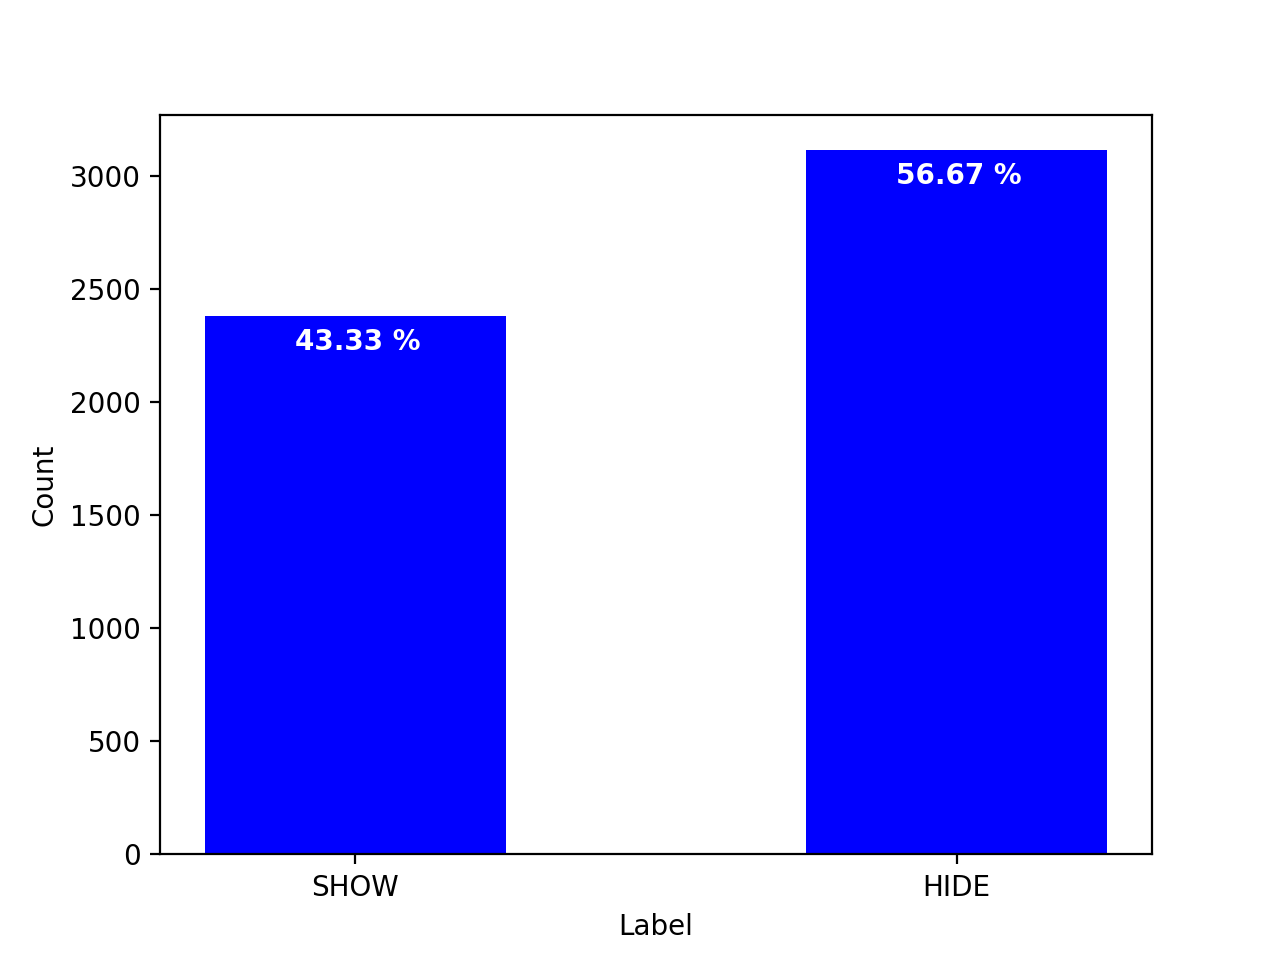
\includegraphics[width=\textwidth]{graphics/labels-dist}
			\end{subfigure}
			\hfill
			\begin{subfigure}{.45\textwidth}
				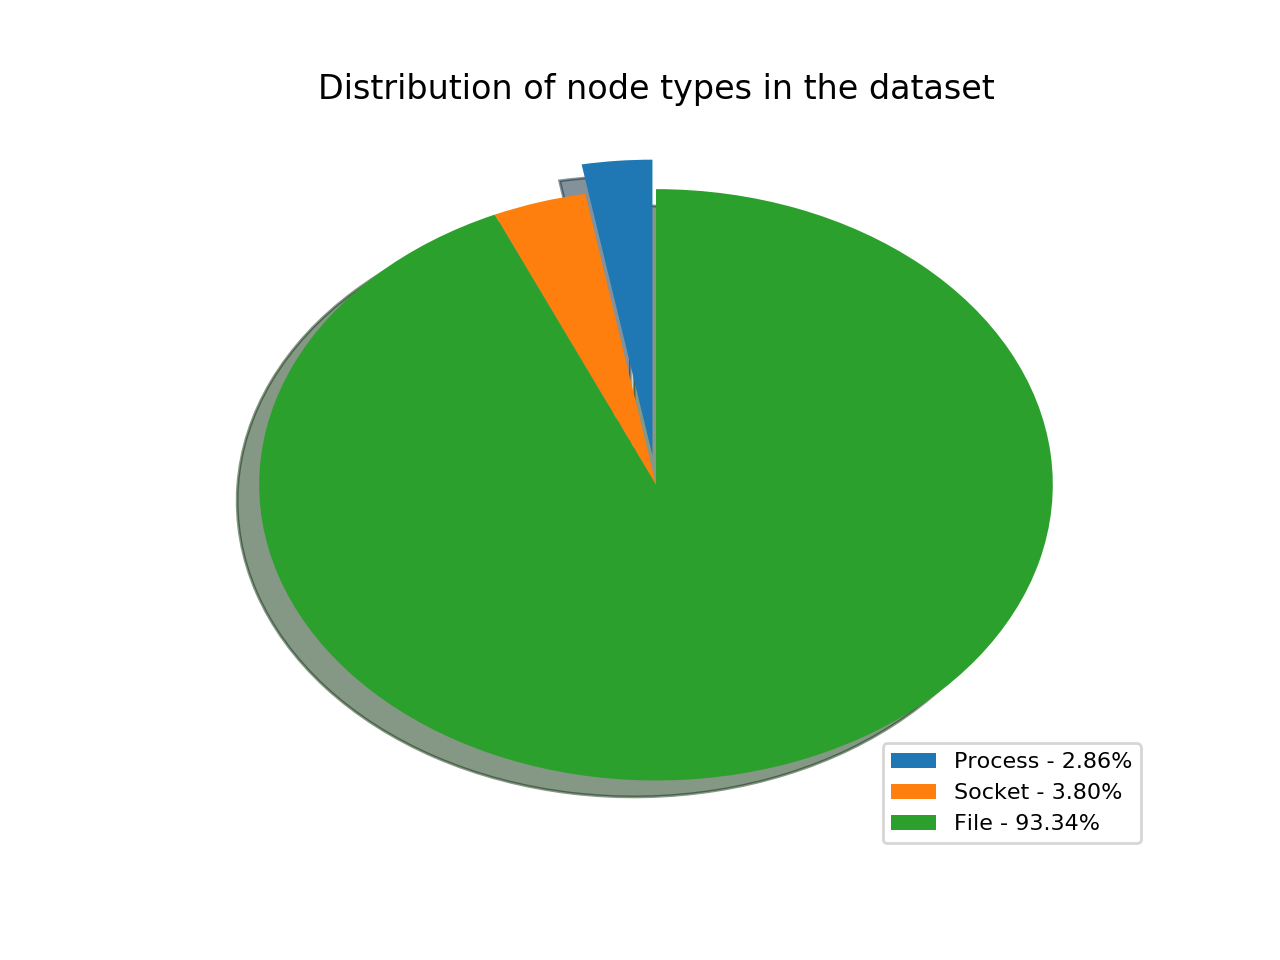
\includegraphics[width=\textwidth]{graphics/node-dist}
			\end{subfigure}
			\caption[Distributions of labels and node type in the dataset]{\textit{Left:} Distribution of the labels in the dataset. \textit{Right: }Distribution of the node types in the dataset.}
			\label{Fig: eval/ml/methodology/dist}
		\end{figure} 
		The technique used when evaluating the models was \textbf{10-fold outer Cross Validation}. Essentially, I split the dataset in $10$ equally-sized slots and use one at a time as a test set, while the other $9$ serve as the training set for the model. Figure \ref{Fig: impl/ml/methodology/kfold/first} shows how the dataset is divided in the first iteration of the cross-validation algorithm. This way, I ensure that none of the models is tested on previously-seen examples and I can correctly asses how well they generalize on the given data.
		\begin{figure}[H]
			\centering
			\includegraphics[width=.8\textwidth]{graphics/k-fold}
			\caption{First step in 10-fold cross validation.}
			\label{Fig: impl/ml/methodology/kfold/first}
		\end{figure}
		
		At every iteration, I compute a set of metrics for estimating the model's performance. The final result for every metric is given by averaging over the values obtained. 
	\subsection{Metrics} \label{Section: eval/ml/metrics}
	
		In this section, I will outline the metrics used when evaluating the machine learning models. The choice of good metrics is essential when comparatively evaluating a number of machine learning models. The simplest metric for evaluating classification algorithms is \textbf{accuracy}: 
		\\
		\begin{equation}
			acc = \frac{\text{no. of correctly predicted nodes}}{\text{total no. of predicted nodes}}
		\end{equation}
		\\
		Accuracy, however, is not efficient when it comes to imbalanced data, as it is the case here (the nodes have a $43\%/57\%$ \textit{SHOW/HIDE} distribution). Therefore, more complex metrics are required in order to correctly assess the performance of the models. These metrics are based on the notions of \textit{true positives, true negatives, false positives} and \textit{false negatives}, which are illustrated through the confusion matrix from Figure \ref{Fig: eval/ml/metrics/confusion-matrix}.
		\begin{figure}[H]
			\centering
			\includegraphics[width=.7\textwidth]{graphics/confusion-matrix}
			\caption{Confusion matrix for two-class classification}
			\label{Fig: eval/ml/metrics/confusion-matrix}
		\end{figure}
		The metrics I used to evaluate the general performance of the models are presented in Table \ref{Table: eval/ml/metrics/metrics}. From those, the F3 score and the MCC are the most meaningful here, ignoring the biased nature of the data. MCC gives a value between $[-1, 1]$, where $1$ represents perfect prediction, $0$ not better than random and $-1$ a total disagreement between the predicted and true labels.
		\begin{longtable}{|p{.15\textwidth}|p{.40\textwidth}|c|}
		   \textbf{Metric} & \textbf{Intuition} &\textbf{Formula} \\
			\hline
			\textit{Precision} & fraction of nodes correctly labelled as \textit{SHOW} in all nodes classified. & {$\centering \text{precision} = \frac{tp}{tp+fp}$} \\
			\hline 
			\textit{Recall} & fraction of \textit{SHOW} nodes correctly classified. & $\text{recall} = \frac{tp}{tp+fn}$ \\
			\hline
			\textit{F3 score} & takes into consideration both the precision and the recall of the model in order to assess its performance. & $\text{F3} = 10\times\frac{\text{precision}\times\text{recall}}{9\times\text{precision} + \text{recall}}$\\
			\hline 
			\textit{Matthew's Correlation Coefficient (MCC)} & takes into account true and false positives and negatives in order to provide a balanced metric for the model's performance. & $MCC = \frac{tp\times tn - fp\times fn}{\sqrt{(tp+fp)\times(tp+fn)\times(tn+fp)\times(tn+fn)}}$\\
			\hline
			\caption{Machine learning evaluation metrics.}
			\label{Table: eval/ml/metrics/metrics}
		\end{longtable}
		
		I chose to use the F3 score instead of the more frequently encountered F1, because it weights the recall of the models more favourably than their precision. I am interested in having a high recall because, in practice, I want the models to show as many of the nodes that are of interest as possible, even if this leads to a lower precision. The F3 score gives a value in $[0, 1]$, with $F3 = 0$ representing a total disagreement between the classification results and the true labels and $F3 = 1$ representing a perfect classification.
		
		\subsection{Results \& discussion} \label{Section: eval/ml/results}
		In this section I will present and discuss the results obtained as part of the models' evaluation. Table \ref{Table: eval/models/results/overall} shows the averaged scores obtained by the four models. 
		
		\begin{longtable}{|p{.15\textwidth}|p{.18\textwidth}|p{.18\textwidth}|p{.18\textwidth}|p{.18\textwidth}|}
			\hline
			& \textbf{Logistic Regression} & \textbf{MLP} & \textbf{PNN} &  \textbf{CNN}\\
			\hline
			\textit{Accuracy} & $91.48 \pm 0.90 \%$ &$91.87 \pm 1.35 \%$  &  $91.94 \pm 1.26 \%$ &\cellcolor{green!50}  $\mathbf{93.74 \pm 6.5 \%}$ \\
			\hline
			\textit{Precision} & $97.81 \pm 0.81\%$& $98.23 \pm 3.41 \%$ &   $89.27 \pm 2.13 \%$ & \cellcolor{green!50} $\mathbf{97.28 \pm 1.10 \%}$  \\
			\hline
			\textit{Recall} & $86.92 \pm 1.60\%$& $86.85 \pm 3.98 \%$ & $92.51 \pm 1.15 \%$ & \cellcolor{green!50} $\mathbf{91.52 \pm 1.51 \%}$  \\
			\hline
			\textit{F3 score} & $87.90 \pm 1.46 \%$ & $87.83 \pm 3.37 \%$  &  $92.17 \pm 1.17 \%$ & \cellcolor{green!50} $\mathbf{92.06 \pm 1.31 \%}$\\
			\hline
			\textit{MCC} & $83.62 \pm 1.65\%$& $84.13 \pm 2.29 \%$ &  $83.70 \pm 2.53 \%$ & \cellcolor{green!50} $\mathbf{87.59 \pm 1.30 \%}$\\
			\hline
			\caption{Evaluation results for the models implemented.}
			\label{Table: eval/models/results/overall}
		\end{longtable}
		From the results above, I can conclude that the CNN is significantly more performant than the others, with \textbf{MCC} $\mathbf{ = 87.59 \pm 1.30 \%}$. Moreover, it has high values for both recall (being very likely to return most of the relevant nodes) and precision (making it an effective filtering algorithm). The PNN has an even higher recall value, classifying more of the relevant nodes as \textit{SHOW}. Its low precision, however, makes it a poor filtering tool, as the analyst would have to search through a larger node space.
		\\ \\
		The bar chart in Figure \ref{Fig: eval/ml/results/MCC-per-fold} illustrates a fold-by-fold breakdown of the MCC results for all 4 models. It supports the previous conclusion, as the CNN has a higher MCC than the other models for $8/10$ folds and therefore generalizes better than them.    
		\begin{figure}[H]
			\centering
			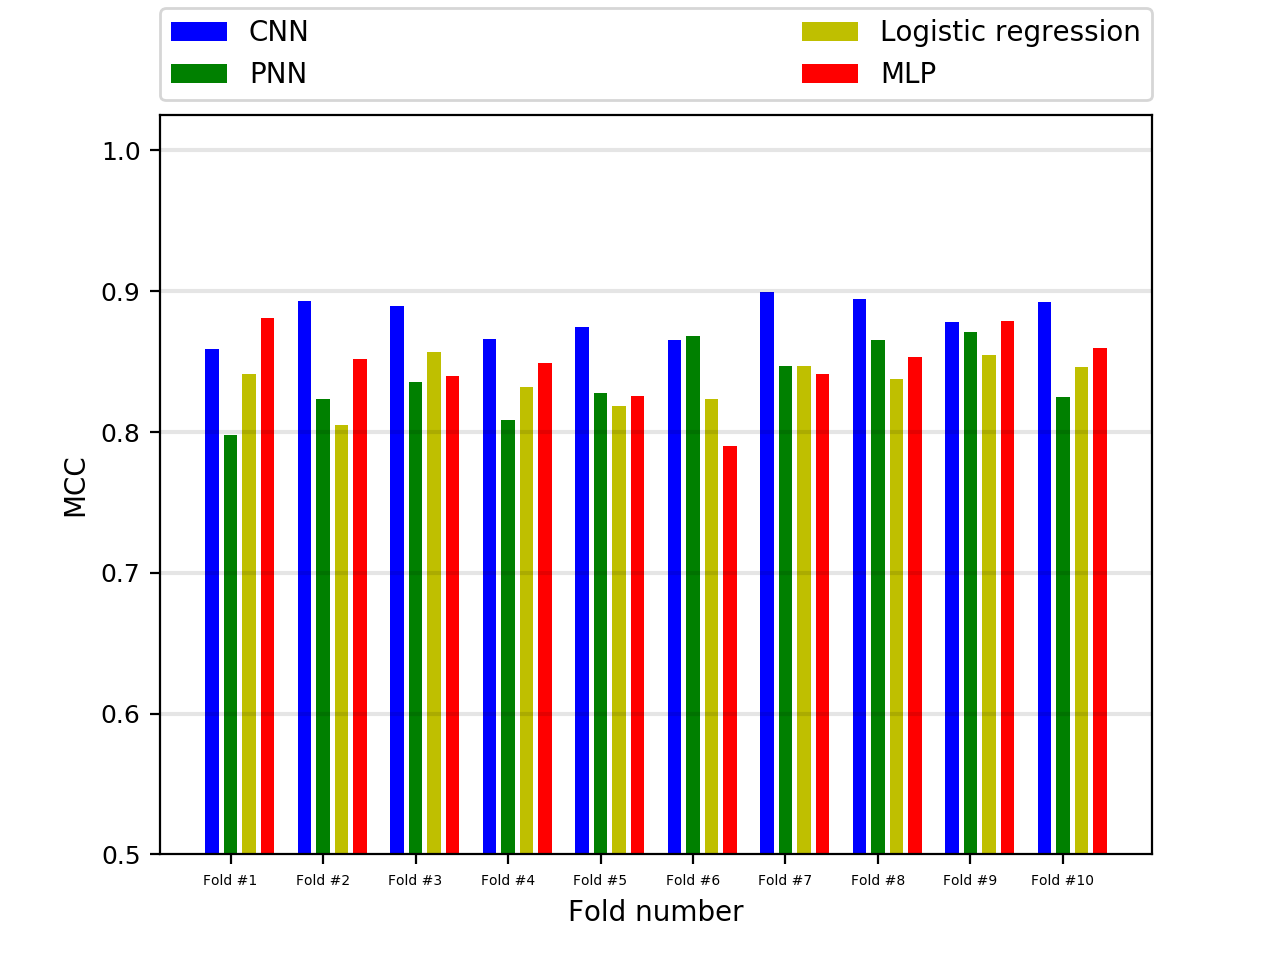
\includegraphics[width=\textwidth]{graphics/MCC-per-fold}
			\caption{Comparative MCC at every fold.}
			\label{Fig: eval/ml/results/MCC-per-fold}
		\end{figure}
		Figure \ref{Fig: eval/ml/results/ROC} illustrates the averaged ROC curves of every model, obtained by interpolating over the 10 folds of the Cross Validation algorithm. The CNN has the steepest ROC curve, indicating that it has the highest ability to discriminate between the two classes ( \textit{SHOW} and \textit{HIDE}). Furthermore, this fact is shown by its ROC-AUC score, which is larger than the one for the other models.
		\begin{figure}[H]
			\centering
			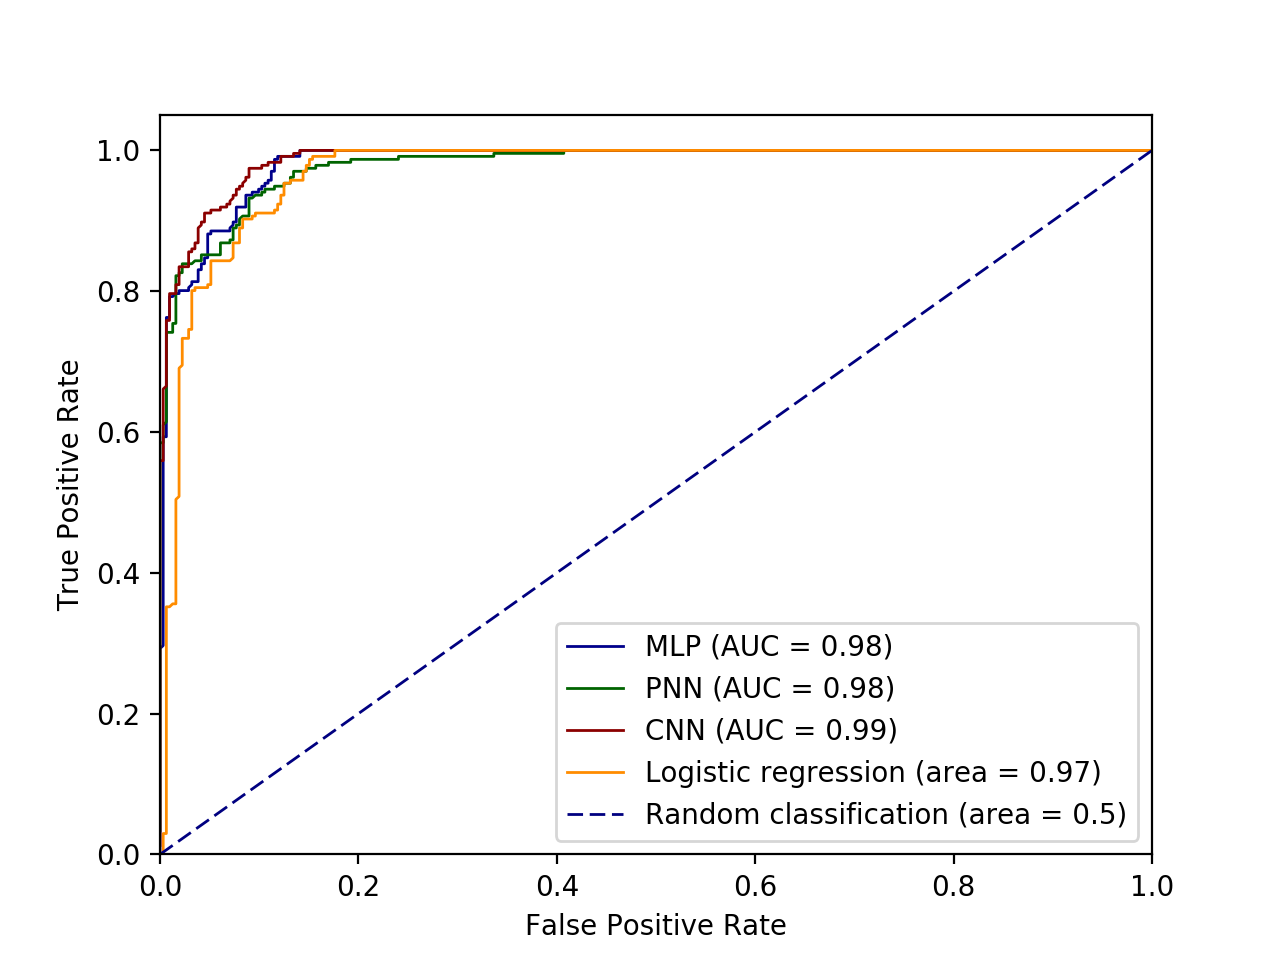
\includegraphics[width=\textwidth]{graphics/ROC-curve}
			\caption{Mean ROC curves obtained after 10-fold outer-CV.}
			\label{Fig: eval/ml/results/ROC}
		\end{figure}
		Concavities present in the curves indicate that, locally, the models have worse than random behaviour and therefore cannot fit the data perfectly. This is a possible consequence of the fact that the models are trying to fit a set of $6$ ground truths in the same time and that some of these rules are fit better than others. 
		\\ \\
		In order to evaluate how well the rules from Section \ref{Section: prep/data/ground-truths} are learned, I first trained the models on the dataset used in the evaluation and then extracted nodes representing each rule from a separate database of $631, 357$ nodes. Figure \ref{Figure: eval/ml/results/per-rule} illustrates the per-rule precision values obtained for every model. Rule 2 (\textit{File that was downloaded and executed}) did not have enough examples in the database to provide comprehensive results and was excluded from this chart. 
		\begin{figure}[H]
			\centering
			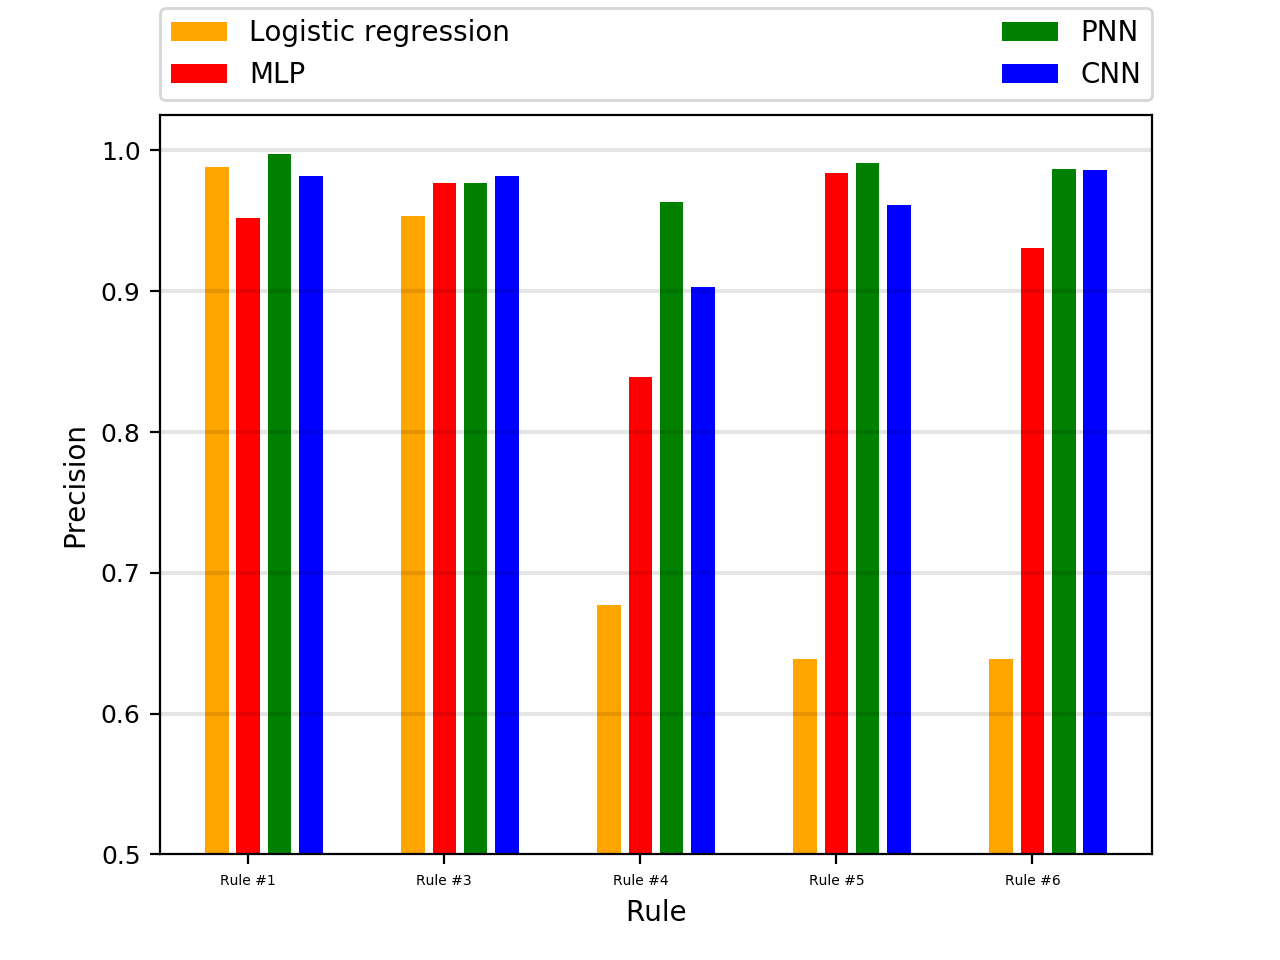
\includegraphics[width=.8\textwidth]{graphics/per-rule-precision}
			\caption{Per-rule precision for the models.}
			\label{Figure: eval/ml/results/per-rule}
		\end{figure}
		By analysing these results, we can conclude that Logistic Regression truly is a weak classifier, failing to fit the rules as expected. While it fits the the $1^{\text{st}}$ and $3^{\text{rd}}$ rule reasonably well, the classifier has a close-to-random behaviour for nodes associated with the last three rules. On the other end of the spectrum, the PNN fits all $5$ rules almost perfectly and the CNN is the second-best, with a minimum precision of $90.32 \%$, obtained for rule $4$ (\textit{Processes that open a Socket to a different machine}).  
		\\ \\
		The precision-recall curves from Figure \ref{Fig: eval/ml/results/precision-recall} show the tradeoff between precision and recall at different probability thresholds for every model. The \textbf{average precision} (AP) summarizes the plots as the weighted mean of precisions:
		\begin{equation}
			AP = \sum_{n} (R_n - R_{n-1}) P_n
		\end{equation}
		where $R_n$ and $P_n$ are the precision and recall at the $n^{th}$ threshold. 
		\\ \\
		From their analysis, we can observe that the CNN(Figure \ref{Fig: eval/ml/results/precision-recall/cnn}) has the highest average precision (AP = $0.98$) and therefore is a highly effective filtering algorithm. The PNN (Figure \ref{Fig: eval/ml/results/precision-recall/pnn}) has a precision close to $1$ for recall values of up to $\approx 0.8$, but then drops steeply, causing a lower value for the average precision (AP = $0.96$). 
		\\ \\
		The other two models also have low AP (i.e. $0.95$ for logistic regression and $0.96$ for MLP), indicating a lower performance. Moreover, the precision-recall curve for logistic regression is highly inconsistent and therefore it is the least performant of the four models. This fits my expectations, as it is the most simplistic model and cannot identify complex relationships between the features I use to represent the nodes.
		\begin{figure}[H]
			\centering
			\begin{subfigure}{.4\textwidth}
				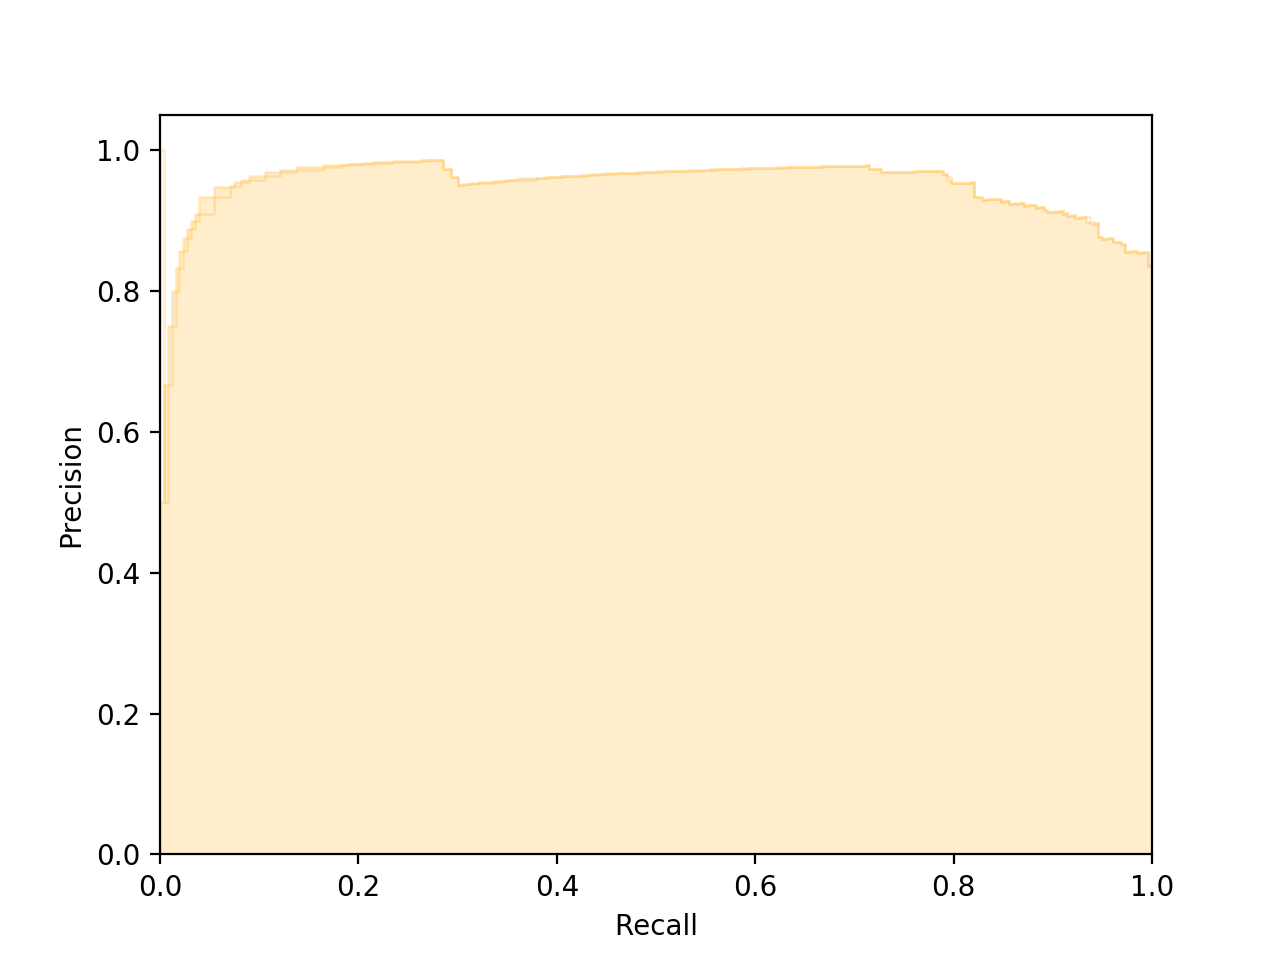
\includegraphics[width=\textwidth]{graphics/precision-recall/logreg}
				\caption{Precision-recall curve for logistic regression. AP = $0.95$}
				\label{Fig: eval/ml/results/precision-recall/logreg}
			\end{subfigure} \hfill
			\begin{subfigure}{.4\textwidth}
				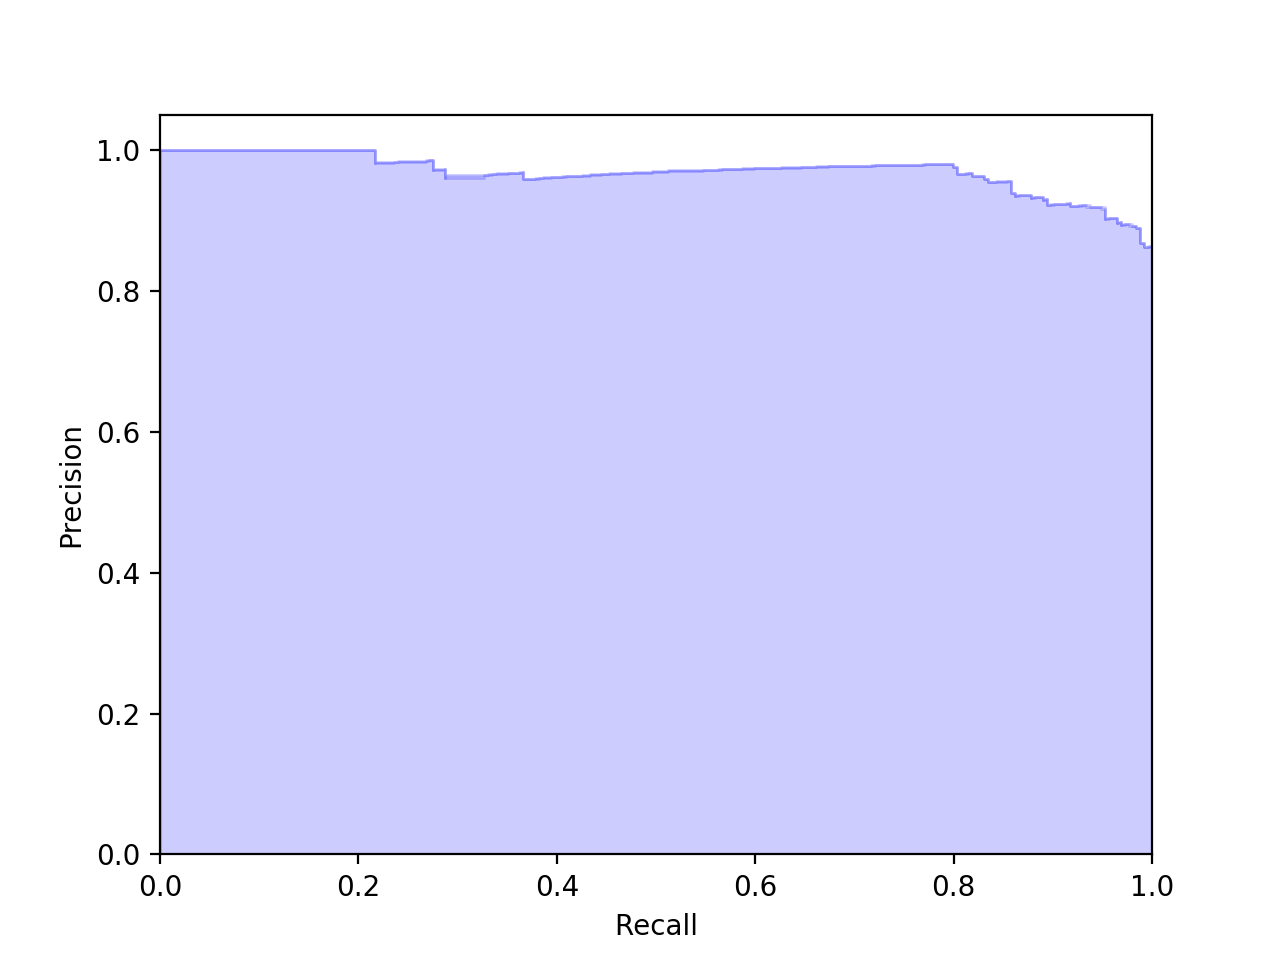
\includegraphics[width=\textwidth]{graphics/precision-recall/mlp}
				\caption{Precision-recall curve for MLP.  AP = $0.96$}
				\label{Fig: eval/ml/results/precision-recall/mlp}
			\end{subfigure}
			\begin{subfigure}{.4\textwidth}
				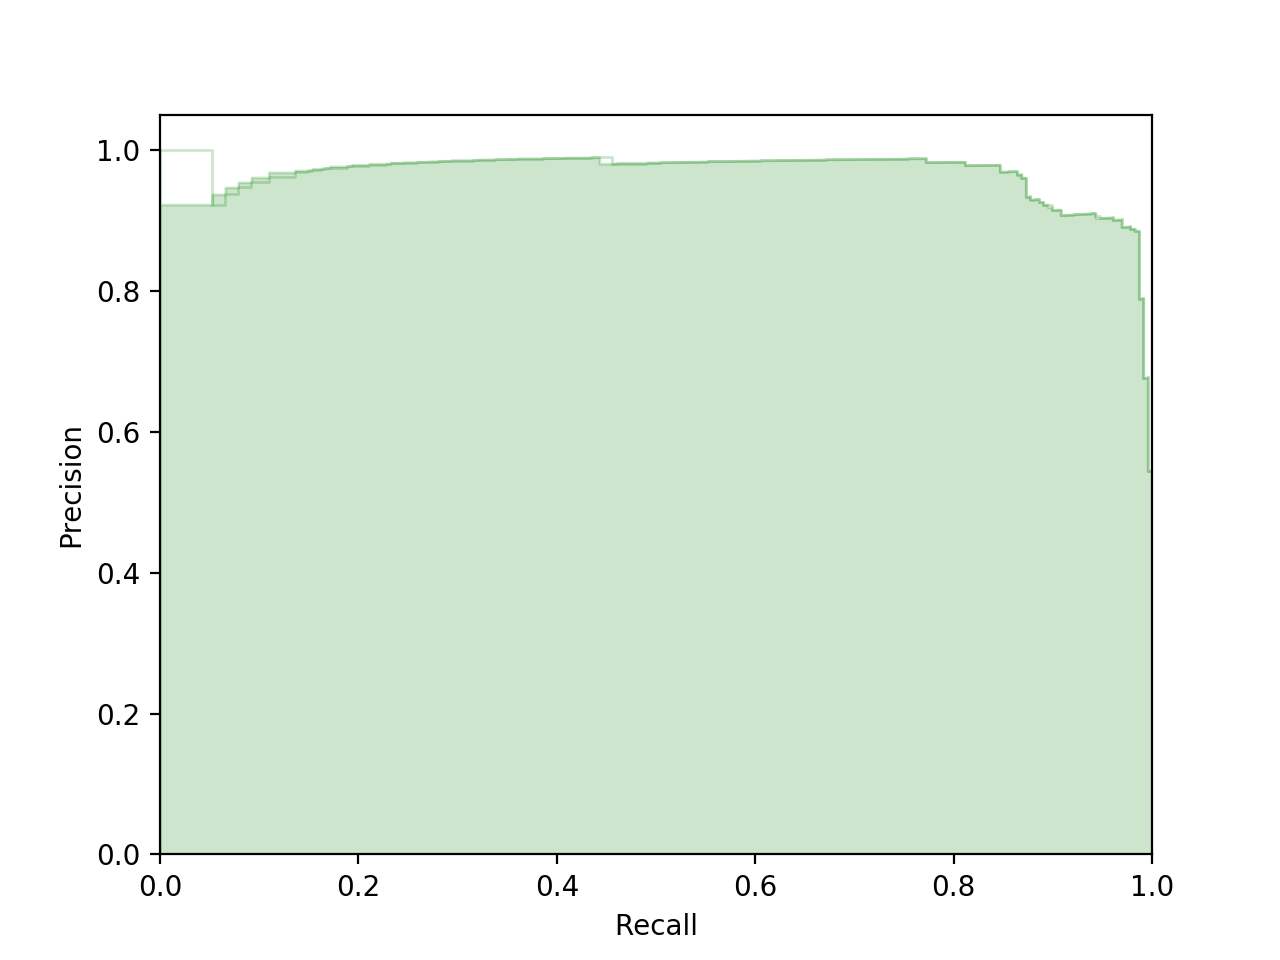
\includegraphics[width=\textwidth]{graphics/precision-recall/pnn}
				\caption{Precision-recall curve for PNN. AP = $0.96$}
				\label{Fig: eval/ml/results/precision-recall/pnn}
			\end{subfigure} \hfill
			\begin{subfigure}{.4\textwidth}
				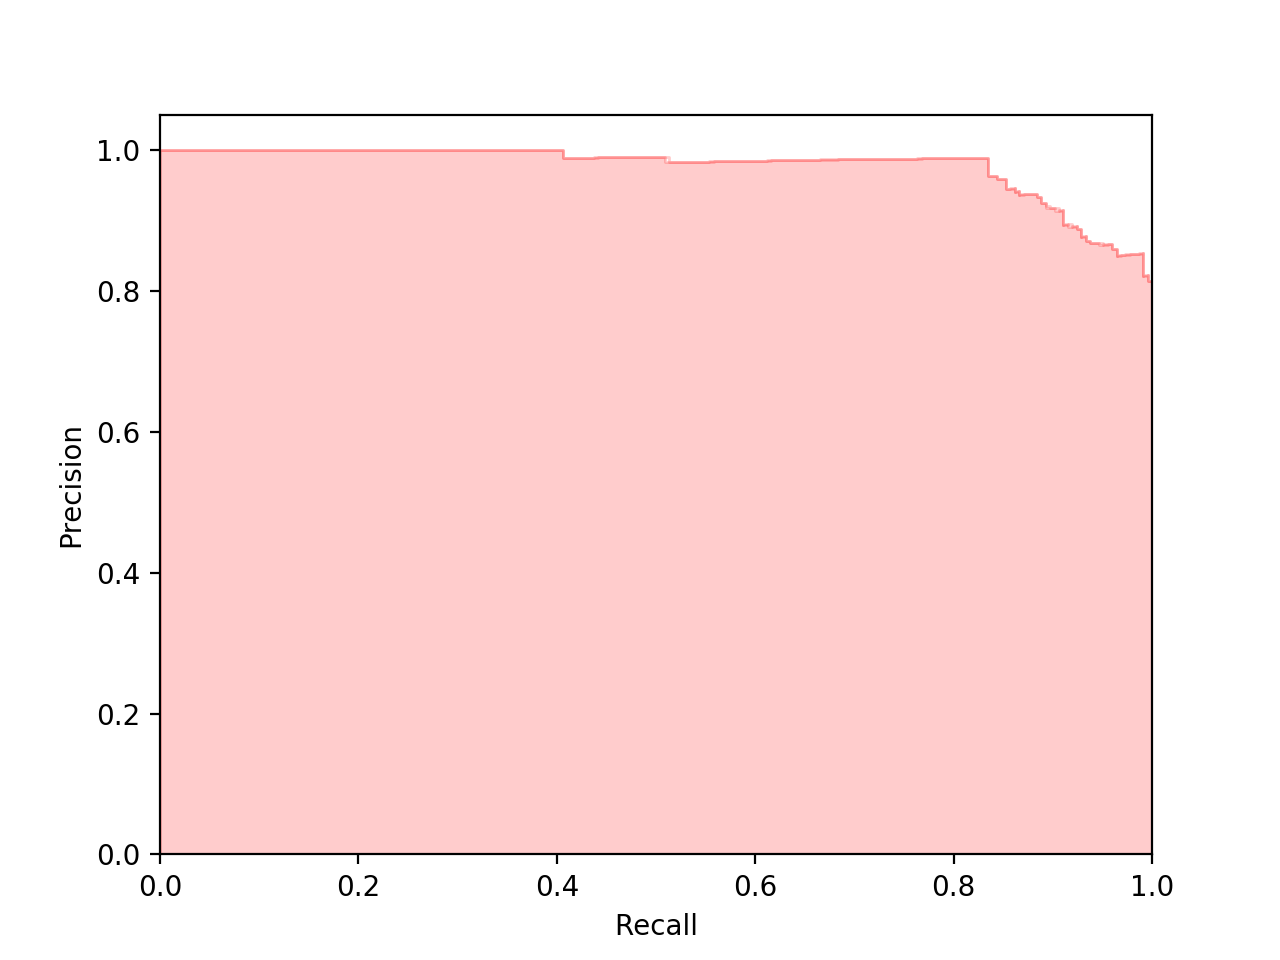
\includegraphics[width=\textwidth]{graphics/precision-recall/cnn}
				\caption{Precision-recall curve for CNN. AP = $0.98$}
				\label{Fig: eval/ml/results/precision-recall/cnn}
			\end{subfigure}
			\caption{Average precision-recall curves for the 4 models.}
			\label{Fig: eval/ml/results/precision-recall}
		\end{figure}
			In conclusion, all four models have a good performance on the data used during evaluation, meeting the success criterion outlined in the Project Proposal (i.e. achieving over $70\%$ in both precision and recall). Although the PNN is best at fitting the ground-truths defined, it has a low  precision, making it less efficient as a filtering algorithm. The CNN, on the other hand, fits the rules almost as well as the PNN and in the same time has the highest overall performance, with  $\text{MCC} = 87.59 \pm 1.30 \%$ and $\text{F3} = 92.06 \pm 1.31 \%$, despite the highly imbalanced data.
			
		\section{Service time evaluation} \label{Section: eval/service-time}
			This project is meant to be a complete API that can be used in practice by the CADETS UI. Therefore, besides the performance of the machine learning models, it is essential to evaluate it in terms of the service speed as well\footnote{All the timing results were obtained using my personal machine.}. For a job processing $N$ nodes, the service time is calculated using the following formula:  
			\begin{equation}
				\text{service\_time} = N\times [CCT + CHR \times CET + (1-CHR) \times (CT + RCT)] + MLT
				\label{Eq: eval/service-time/overall}
			\end{equation}
			where: 
			\begin{itemize}
				\item $\mathbf{CCT} \in \mathbb{R}$ = Cache Check Time - time for checking if a node has a valid cache entry.
				\item $\mathbf{CHR} \in [0, 1]$ = Cache Hit Rate.
				\item $\textbf{CET} \in \mathbb{R}$ = Cache Extraction Time - time for extracting a cached result.
				\item $\textbf{CT} \in \mathbb{R}$ = Classification Time - time for classifying a node. 
				\item $\textbf{RCT} \in \mathbb{R}$ = Result Caching Time - time for adding a classification result to the cache database.
				\item $\mathbf{MLT} \in \mathbb{R}$ = Model Loading Time - time for configuring the model (i.e. defining its components and loading the pre-optimised parameters).
			\end{itemize}
			In practice, the API is expected to re-use many of the classification results. For this reason, I assume $CHR = 90\%$. For simulation purposes, the database was populated with $10, 000$ nodes and $30$ completed jobs, each having processed $1, 000$ nodes. 
			\\ \\
			The first step when a new job is initiated is to check the cache and extract the nodes that have a valid cache entry. In this simulation environment, the Cache Check Time, Cache Extraction Time and Result Caching Time are $CCT=0.01s$, $CET=0.02s$ and $RCT=0.01s$, respectively.  
			
		\subsection{Classification timings} \label{Section: eval/service-time/classification}
			The classification time is not as straight-forward as the times shown so far. It was computed using the following formula:
			\begin{equation}
				CT = NTT + FET + MRT
			\end{equation}
			where: 
			\begin{itemize}
				\item $\mathbf{NTT} \in \mathbb{R}$ = Node Type Time - time for getting the node type.
				\item $\mathbf{FET} \in \mathbb{R}$ = Feature Extraction Time - time for extracting the features required for a node.
				\item $\mathbf{MRT} \in \mathbb{R}$ = Model Running Time - time for producing a classification result for a node.
			\end{itemize}
			If a node is not in the cache, we first need to get its type. The feature extraction time is dependent on this, as different node types require a slightly different feature extraction algorithm. Moreover, for a \textit{Pipe} node, we also need to look for the closest \textit{Process} node to it. Table \ref{Table: eval/service-time/classification/fet} shows a breakdown of these timings\footnote{The time values were estimated by averaging over 100 runs of the feature extractor, with 20 nodes each.}, when the nodes are extracted from a database of $6,008$ nodes and taking into account the policy defined in Section \ref{Section: impl/REST/actual}.
			\begin{longtable}{|p{.1\textwidth} || p{.15\textwidth} | p{.20\textwidth}| p{.15\textwidth}| p{.20\textwidth} | }
				\textbf{Node type} & \textbf{NTT} (s) & \textbf{Time for finding the closest node} (s)& \textbf{FET} (s)& \textbf{Total FET} (s)\\
				\hline
				\textit{File} & \multirow{5}{*}{$0.13$}& $0.0$ & $0.78$& $\mathbf{0.91}$ \\
				\hhline{-~---}
				\textit{Process} & & $0.0$ & $0.83$ & $\mathbf{0.96}$\\
				\hhline{-~---}
				\textit{Socket} & & $0.0$ & $0.67$ & $\mathbf{0.80}$ \\
				\hhline{-~---}
				\textit{Pipe} & & $0.01$ & $0.83$ & $\mathbf{0.97}$ \\
				\hhline{-~---}
				\textit{Machine} & & $0.0$ & $0.0$ & $\mathbf{0.13}$\\
				\hline
				\caption{Breakdown of feature extraction times}
				\label{Table: eval/service-time/classification/fet}
			\end{longtable}		
			Once the feature vectors are computed, they are passed to the machine learning models to be classified. Depending on the model type, this task can take different amounts of time. The classification time can be written as a function of node and model type as follows: 
			\begin{equation}
				CT(nt, mt) = Total\_FET(nt) + MRT(mt)
			\end{equation}
			Considering the node type distribution outlined in the histogram from Figure \ref{Figure 2.1.1}, the average feature extraction time can be calculated as follows:
			\begin{equation}
				\hat{FET} = \sum_{nt\in \mathbf{\mathcal{N}}} (\mathbb{P}(nt) \times Total\_FET(nt))
			\end{equation} 
			where $\mathcal{N}$ is the set of node types. By plugging in the numbers, $\hat{FET} = 0.89\text{s}$. Using this, the average classification time as a function of model type is: 
			\begin{equation}
				\hat{CT}(mt) =  \hat{FET} + MRT(mt) 
			\end{equation}  
			 Table \ref{Table: eval/service-time/classification/CT} shows the resulting $MLT$, $MRT$  and $\hat{CT}$ for each model.
			
			\begin{longtable}{|p{.15\textwidth}||p{.15\textwidth}|p{.15\textwidth}|p{.15\textwidth}|p{.15\textwidth}|}
				\textbf{Model} & \textit{Logistic Regression} & \textit{MLP} & \textit{CNN} & \textit{PNN} \\
				\hline
				$\mathbf{MLT}$ (s) & $0.01$ & $0.02$ & $0.02$ & $0.01$  \\
				\hline
				$\mathbf{MRT}$ (s) & $0.01$ &$0.01$ & $0.01$ & $0.09$ \\
				\hline\hline
				$\mathbf{\hat{CT}}$ (s) & $\mathbf{0.90}$ & $\mathbf{0.90}$ & $\mathbf{0.90}$ & $\mathbf{0.99}$ \\
				\hline
				\caption{Breakdown of average classification times.}
				\label{Table: eval/service-time/classification/CT}
			\end{longtable} 
			
			\subsection{Bringing it all together} \label{Section: eval/service-time/together}
			Now that I computed all the individual times, I can bring them all together and compute the \textit{service time}, using Eq. \ref{Eq: eval/service-time/overall}. Table \ref{Table: eval/service-time/together/overall} shows the resulting service times for different models, for $N=1,000$ nodes.
			\begin{longtable}{|p{.13\textwidth}||p{.08\textwidth}|p{.08\textwidth}|p{.08\textwidth}|p{.08\textwidth}|p{.08\textwidth}|p{.08\textwidth}|p{.08\textwidth}||p{.1\textwidth}|}
				\textbf{Model} & \textbf{N} & \textbf{CHR}  &\textbf{CCT} (s) & \textbf{CET} (s) & \textbf{RCT} (s)& $\mathbf{\hat{CT}}$ (s)& \textbf{MLT} (s) & \textbf{Total} (s)\\
				\hline
				\textit{Logistic Regression} & \multirow{5}{*}{$1000$} & \multirow{5}{*}{$0.90$} & \multirow{5}{*}{$0.01$} & \multirow{5}{*}{$0.02$} & \multirow{5}{*}{$0.01$} & $0.90$ & $0.01$ & \cellcolor{green!20} $\mathbf{119.01}$ \\
				\hhline{-~~~~---}
				\textit{MLP} &  &  &   & &  & $0.90$ & $0.02$ &\cellcolor{green!20} $\mathbf{119.02}$  \\
				\hhline{-~~~~---}
				\textit{CNN} &  &  &  & &  & $0.90$ & $0.02$ & \cellcolor{green!20} $\mathbf{119.02}$ \\
				\hhline{-~~~~---}
				\hhline{-~~~~---}
				\textit{PNN} &  &  &  & &  & $0.99$ & $0.01$ & \cellcolor{green!20} $\mathbf{128.01}$ \\
				\hline
				\caption{Service time analysis results.}
				\label{Table: eval/service-time/together/overall}
			\end{longtable}
			
			From these results we can observe that there is little difference between the models when it comes to the API's overall running time. For the PNN, the API takes the most time to run. This is a consequence of the fact that the number of vector operations that need to be performed is directly proportional to the number of training samples provided, unlike the other models, which all have a constant number of neurons. 
			\\ \\
			Another key observation is the fact that the classification time $\hat{CT}$ has the highest impact on the service time. To be precise, the feature extraction step is the most impactful in this case. This is caused by the poor performance of the external library used to connect to the Neo4J database and represents a significant bottleneck for the API's performance. In order to overcome this issue, I decided to use a cache database, by relying on the fact that the classification results are unlikely to change over time. In order to better illustrate the impact of the caching mechanism, I first define the service time formula for a non-caching API:
			\begin{equation}
				service\_time = N \times \hat{CT} + MLT
			\end{equation}
			Based on this formula and the results above, I plotted the bar chart from Figure \ref{Fig: eval/service-time/bringing/bar}, which illustrates the difference in service time between a caching API and an API that just classifies every node for a request. From it we can observe that, when using a cache, the API is several orders of magnitude more time efficient than the non-caching version. Therefore, the cache database is an efficient solution for overcoming the bottleneck posed by the feature extraction step.  
			\begin{figure}[H]
				\centering
				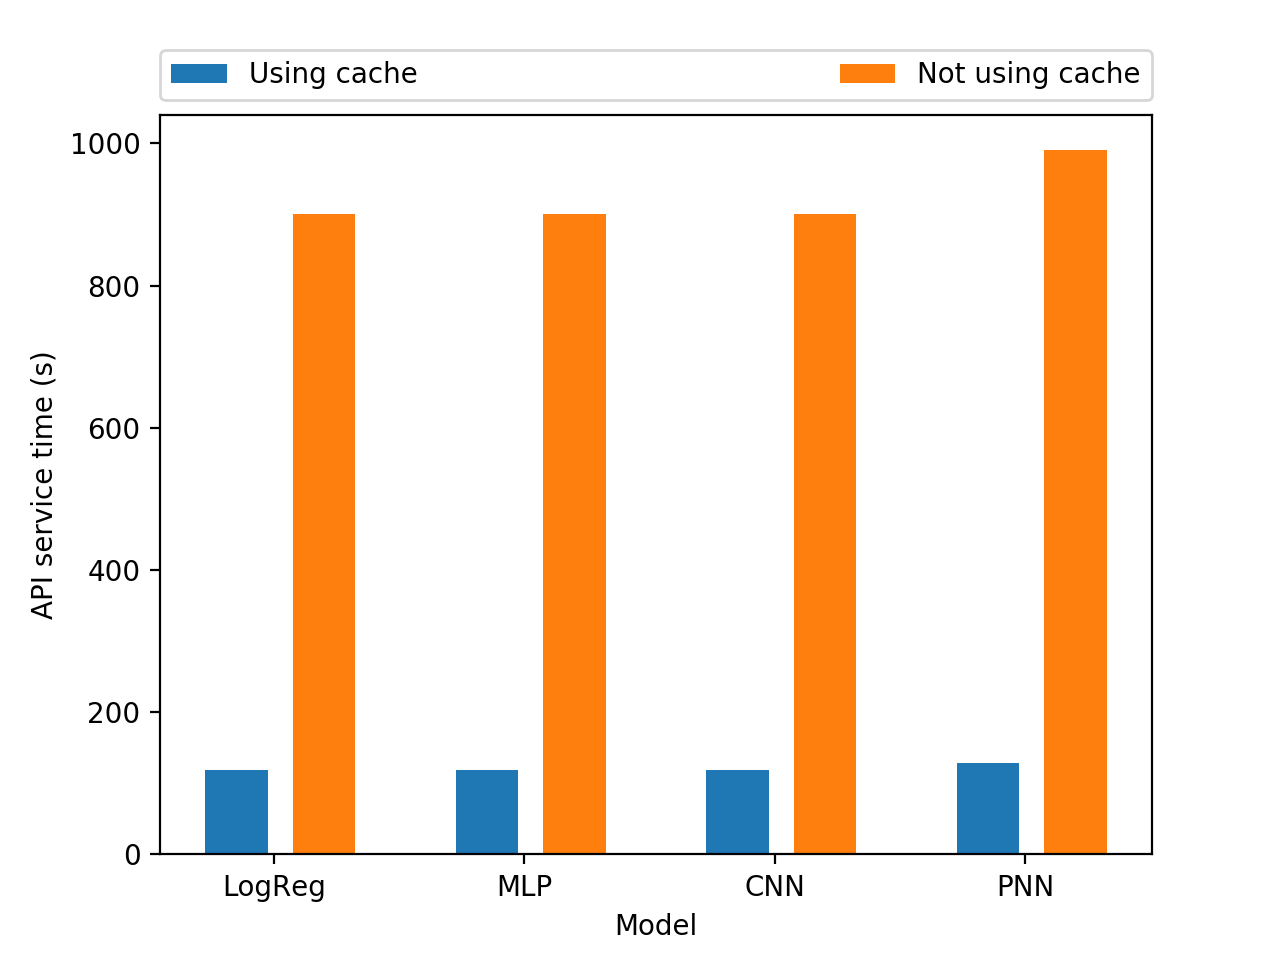
\includegraphics[width=.7\textwidth]{graphics/service-time-hist}
				\caption{Service times with/ without using cache for $N=1,000$ nodes and $CHR=0.90$.}
				\label{Fig: eval/service-time/bringing/bar}
			\end{figure}
			Even though the cache database partially solves the feature extractor limitation, the service time of the API is still high. For this reason, I decided to implement the 2-step format of the API described in Section \ref{Section: impl/REST/actual}.
		\section{Summary} \label{Section: eval/summary}
			Initially, this chapter listed the success criteria for this project and how they were achieved. Following this, I described how the models implemented met the expected performance and, through comparative evaluation, shown the fact that the CNN outperforms the other models on the dataset described in Section \ref{Section: eval/ml/methodology}. In the end, I evaluated the tool from a service-time point of view and highlighted the bottlenecks encountered and which motivated some of my implementation decisions. 
\end{document}